\documentclass[twoside]{book}
\newif\ifpdf
\ifx\pdfoutput\undefined
\pdffalse % we are not running PDFLaTeX
\else
\pdfoutput=1 % we are running PDFLaTeX
\pdftrue
\fi
%\usepackage{times}
%\usepackage{amsmath}
\usepackage{calc}
\usepackage[latin1]{inputenc}
\usepackage{FFF}
\usepackage{amsfonts}
\usepackage{amsmath}
\usepackage{hyperref}
\usepackage{FFF}
\usepackage{makeidx}
\usepackage{color}
\usepackage{multicol}
\usepackage{graphicx}
%\usepackage{dessin}
\topmargin -1.54cm
\oddsidemargin 0cm   %marge a 2 cm
\evensidemargin 0cm  %marge a 2 cm
\newcommand{\indente}{\hbox to \parindent {\hss}}
\parindent 0cm
\headsep 0.5cm
\topskip .5cm
\footskip 1cm
\headheight 1.0cm
\textwidth  16.5cm
%  \parindent 0cm
\textheight 24cm
\def\freefempp{\texttt{freefem++ }}
\def\textRed{\color{red}}
\def\textBlack{\color{black}}
\def\Blue#1{\textcolor{blue}{#1}}
\def\Black#1{\textcolor{black}{#1}}
\def\Red#1{\textcolor{red}{#1}}
\def\Magenta#1{\textcolor{magenta}{#1}}
\def\hin{\hbox{ in }}
\def\hon{\hbox{ on }}
\def\Cpp{\texttt{C++~}}
\def\R{\mathrm{I\!R}}
\def\example{\textbf{Example:}}
\def\eq#1{\Blue{\[#1\]}}
\def\R{\mathbb{R}}
\def\Z{\mathbb{Z}}
\def\itemtt[#1]{ \item[\texttt{#1}]}
\def\plot[#1]#2#3{\begin{figure}[hbt]
\begin{center}
    \includegraphics*[#1]{#2}
\end{center}
\caption{\label{#2} #3}
\end{figure}
}
\def\Ostream{\texttt{ostream}}
\def\Istream{\texttt{istream}}
\def\Bool{\texttt{bool}}
\def\Real{\texttt{real}}
\def\Int{\texttt{int}}
\def\vecttwo#1#2{\left|\begin{smallmatrix} #1 \\ #2 \end{smallmatrix}\right.}
\def\vdeux(#1,#2){\left|\begin{smallmatrix} #1 \\ #2 \end{smallmatrix}\right.}
\def\HLINE#1{\hbox to \hsize {#1}}
\def\twoplot[#1]#2#3#4#5{
\begin{figure}[hbt]
\begin{multicols}{2}
\begin{center}
    \includegraphics*[#1]{#2}
    \caption{\label{#2} #4}
\end{center}
\begin{center}
    \includegraphics*[#1]{#3}
    \caption{\label{#3} #5}
\end{center}
\end{multicols}
\end{figure}
}% end twoplot macro
\newtheorem{remark}{\textbf{Remark}}
\newtheorem{bug}{\textbf{Bug:}}
\newtheorem{proposition}{\textbf{Proposition}}
\newtheorem{algorithm}{\textbf{Algorithm}}
\newenvironment{ttlist}
   {\begin{list}{}{\renewcommand{\makelabel}[1]{\texttt{##1}\hfil}%
        \setlength{\labelwidth}{3cm}
        \setlength{\leftmargin}{\labelwidth+\labelsep}
    }}%
   {\end{list}}


\begin{document}
\graphicspath{{./}{plots/}}
\ifpdf
\DeclareGraphicsExtensions{.pdf, .jpg, .tif}
\else
\DeclareGraphicsExtensions{.eps,.ps, .jpg}
\fi

\let\subsubsection\subsection
\let\subsection\section
\let\section\chapter




\textBlack
The nonlinear elasticity  problem is find  the deplacement $(u_{1},u_{2})$  minimizing  $J$
$$ \min J(u_{1},u_{2}) = \int_{\Omega} f(F2) -  \int_{\Gamma_{p}} P_{a} \,  u_{2} $$
where  $F2(u_{1},u_{2}) =  A(E[u_{1},u_{2}],E[u_{1},u_{2}])$ and $A(X,Y)$ is bilinear sym. positive form with respect two matrix $X,Y$.
where $f$ is a given $\mathcal{C}^2$  function, and $E[u_{1},u_{2}] = (E_{ij})_{i=1,2,\,j=1,2}$ is the Green-Saint Venant deformation tensor defined  with: 
$$  E_{ij} = 0.5 ( \partial_i u_j + \partial_j u_i ) + \sum_k \partial_i u_k \times \partial_j u_k  $$ 



The differential of $J$ is 
  $$ DJ(u_{1},u_{2})(v_{1},v_{2}) = \int 2 A(E[u_{1},u_{2}],DE[u_{1},u_{2}](v_{1},v_{2})) f'(F2(u_{1},u_{2}))) -  \int_{\Gamma_{p}} P_{a}  u_{2}  $$

denote $\mathbf{u}=u_{1},u_{2}$, $\mathbf{v}=v_{1},v_{2}$, $\mathbf{w}=(w_{1},w_{2})$ and  
the second order differential is
 {\begin{eqnarray*}
D^2 J(\mathbf{u})((\mathbf{v}),(\mathbf{w}))  &= & A(E[\mathbf{u}],DE[\mathbf{u}](\mathbf{v})) A(E[\mathbf{u}],DE[\mathbf{u}](\mathbf{w})) f''(F2(\mathbf{u}))) \\
 & + &  A(DE[\mathbf{u}](\mathbf{v}),DE[\mathbf{u}](\mathbf{w})) f'(F2(\mathbf{u}))) \\
 &+&  A(DE[\mathbf{u}],D^{2}E[\mathbf{u}]((\mathbf{v}),(\mathbf{w}))) f'(F2(\mathbf{u}))) 
\end{eqnarray*}}
 where $DE$ and $D^{2}E$ are the first and second differential of $E$.
 
 \medskip

The Newton Method is

choose $ n=0$,and $u_O,v_O$ the initial displacement 
\begin{itemize}
\item loop: \par
\item  \hspace{1cm}    find $(du,dv)$ :  solution of 
$$ D^2J(u_n,v_n)((w,s),(du,dv)) =  DJ(u_n,v_n)(w,s) , \quad \forall w,s $$
\item  \hspace{1cm}      $un =un - du,\quad vn =vn - dv$ 
\item  \hspace{1cm}      until $(du,dv)$ small is enough
\end{itemize}

\color{black}The way to implement this algorithme in \freefempp is
use a macro tool to implement  $A$ and $F2$, $f$, $f'$,$f''$.

A macro\label{macro}\index{macro} is like is \texttt{ccp} preprocessor of \Cpp, but this begin by 
\texttt{macro} and the end of the macro definition is the begin of the comment $//$.
In this case the macro is very useful because the type of parameter can be change. 
And  it is easy to make automatic differentiation.

\bFF  

//  non linear elasticity model \hfilll
//   \hfilll
//  -------------------------------\hfilll
//  with huge utilisation of  macro\hfilll
// ---------------------------\hfilll
//   optimize version \hfilll
// ------------\hfilll
//  problem is  find $(uu,vn)$  minimizing  $J$\hfilll
//  $ min J(un,vn) = int f(F2) -  int Pa * un $\hfilll
//   $ dJ(u,u,uu,vv) = int dF2(u,v,uu,vv) df(F2(u,v))$ \hfilll
//   where $F2 =  (^t {E}  A {E} )$ , \hfilll
//   $E(U) =  1/2 (\nabla U + \nabla U^t + \nabla U^t  \nabla U) $ \hfilll
//         ($u_1$) \hfilll
//  with U=(   )\hfilll
//         ($u_2$)\hfilll
// so: \hfilll
// \hfilll$$ E_{ij} = 0.5 ( d_i u_j + d_j u_i ) + \sum_k d_i u_k * d_j*u_k  \leqno(1)$$ 
//  the 3 componantes of the Green Saint Venant deformation tensor: \hfilll
//  $E1(u1,u2) =    E_{11} $\hfilll
//  $E2(u1,u2) =    E_{12} = E_21 $\hfilll
//  $E3(u1,u2) =    E_{22}  $\textBlack\hfilll
\eFF

\bFF

// remark : we can parametrize E1,E2,E3 with:\hfilll
//  EE(da,db,a,b,u1,u2) \hfilll
//   where $da,db$ correspond to $d_i, d_j$ in (1)\hfilll
//   where  $a,b$  correspond to $u_i, u_j$ in (1)\hfilll
//   where $u1,u2$  correspond to $u_1, u_2$ in (1)\hfilll
//  ----------------------------------------------

//  first the linear part of EE linear elasticite\hfilll
// remark a macro end with a // comment \hfilll
macro EEL(di,dj,ui,uj) ( (di(uj)+dj(ui))*0.5 )    // 11

// non linear par of EE (bilinear)  simple to differential \hfilll
macro bEENL(di,dj,u1,u2,v1,v2) (di(u1)*dj(v1)*.5+di(u2)*dj(v2)*0.5) 
// 
macro EENL(di,dj,u1,u2) bEENL(di,dj,u1,u2,u1,u2) // 
macro dEENL(di,dj,u1,u2,du1,du2) ( bEENL(di,dj,du1,du2,u1,u2) 
                                  + bEENL(di,dj,u1,u2,du1,du2) )   
//   ------------ \hfilll
macro EE(di,dj,ui,uj,u1,u2) (EEL(di,dj,u1,uj) + EENL(di,dj,u1,u2)) //
macro dEE(di,dj,dui,duj,u1,u2,du1,du2) (EEL(di,dj,du1,duj) 
                                         + dEENL(di,dj,u1,u2,du1,du2)) //
macro ddEE(di,dj,du1,du2,ddu1,ddu2) ( dEENL(di,dj,du1,du2,ddu1,ddu2)) 
//
// remark  : \hfilll
// $ dEE(di,dj,dui,duj,u1,u2,du1,du2)$  is "the formal differential of EE" \hfilll
// where $du1=\delta u1$ ,$du2=\delta u2$ \hfilll
// $ ddEE(di,dj,dui,duj,u1,u2,du1,du2)$  is "the formal differential of dEE" \hfilll
// where $ddu1=\delta^2 u1$ ,$ddu2=\delta^2 u2$ \hfilll
// --- \hfilll

//  the macro corresponding to the 3 componante of E \hfilll
macro E1(u,v)  /*E11*/EE(dx,dx,u,u,u,v)  //
macro E2(u,v)  /*E12*/EE(dx,dy,u,v,u,v)  //
macro E3(u,v)  /*E22*/EE(dy,dy,v,v,u,v)  //

macro dE1(u,v,uu,vv) /*dE11*/dEE(dx,dx,uu,uu,u,v,uu,vv) // 
macro dE2(u,v,uu,vv) /*dE12*/dEE(dx,dy,uu,vv,u,v,uu,vv) //
macro dE3(u,v,uu,vv) /*dE22*/dEE(dy,dy,vv,vv,u,v,uu,vv) //
macro ddE1(u,v,uu,vv,uuu,vvv) /*ddE11*/ddEE(dx,dx,uu,vv,uuu,vvv) //
macro ddE2(u,v,uu,vv,uuu,vvv) /*ddE12*/ddEE(dx,dy,uu,vv,uuu,vvv) //
macro ddE3(u,v,uu,vv,uuu,vvv) /*ddE22*/ddEE(dy,dy,uu,vv,uuu,vvv) 
//
//  a formal bilinear term \hfilll
macro PP(A,B,u,v) (A(u,v)*B(u,v)) 
// 
// a formal diff  bilinear term \hfilll
macro dPP(A,B,dA,dB,u,v,uu,vv) (dA(u,v,uu,vv)*B(u,v) + A(u,v)*dB(u,v,uu,vv)) 
//
// a formal $diff^2$ bilinear term \hfilll

macro ddPP(A,B,dA,dB,ddA,ddB,u,v,uu,vv,uuu,vvv) (
  dA(u,v,uu,vv)*dB(u,v,uuu,vvv) + dA(u,v,uuu,vvv)*dB(u,v,uu,vv) 
  +  ddA(u,v,uu,vv,uuu,vvv)*B(u,v) + A(u,v)*ddB(u,v,uu,vv,uuu,vvv) 
  ) //
// so the @matrix A is 6 coef \hfilll
//      
//     a11 a12 a13 \hfilll
//     a12 a22 a23 \hfilll
//     a13 a23 a33 \hfilll
macro F2(u,v)  /* F2 */  (
     a11*PP(E1,E1,u,v)
  +  a22*PP(E2,E2,u,v)
  +  a33*PP(E3,E3,u,v)
  +  a13*PP(E1,E3,u,v)
  +  a13*PP(E3,E1,u,v)
  +  a12*PP(E1,E2,u,v)
  +  a12*PP(E2,E1,u,v)
  +  a23*PP(E2,E3,u,v)
  +  a23*PP(E3,E2,u,v)
)  // end macro F2

macro dF2(u,v,uu,vv)  /* dF2 */  (
       a11*dPP(E1,E1,dE1,dE1,u,v,uu,vv)
     + a12*dPP(E1,E2,dE1,dE2,u,v,uu,vv)
     + a13*dPP(E1,E3,dE1,dE3,u,v,uu,vv)
     + a21*dPP(E2,E1,dE2,dE1,u,v,uu,vv)
     + a22*dPP(E2,E2,dE2,dE2,u,v,uu,vv)
     + a23*dPP(E2,E3,dE2,dE3,u,v,uu,vv)
     + a31*dPP(E3,E1,dE3,dE1,u,v,uu,vv)
     + a32*dPP(E3,E2,dE3,dE2,u,v,uu,vv)
     + a33*dPP(E3,E3,dE3,dE3,u,v,uu,vv)
) // end macro dF2 ($D F2$)

macro ddF2(u,v,uu,vv,uuu,vvv)  /* ddF2 */  (
       a11*ddPP(E1,E1,dE1,dE1,ddE1,ddE1,u,v,uu,vv,uuu,vvv)
     + a12*ddPP(E1,E2,dE1,dE2,ddE1,ddE2,u,v,uu,vv,uuu,vvv)
     + a13*ddPP(E1,E3,dE1,dE3,ddE1,ddE3,u,v,uu,vv,uuu,vvv)
     + a21*ddPP(E2,E1,dE2,dE1,ddE2,ddE1,u,v,uu,vv,uuu,vvv)
     + a22*ddPP(E2,E2,dE2,dE2,ddE2,ddE2,u,v,uu,vv,uuu,vvv)
     + a23*ddPP(E2,E3,dE2,dE3,ddE2,ddE3,u,v,uu,vv,uuu,vvv)
     + a31*ddPP(E3,E1,dE3,dE1,ddE3,ddE1,u,v,uu,vv,uuu,vvv)
     + a32*ddPP(E3,E2,dE3,dE2,ddE3,ddE2,u,v,uu,vv,uuu,vvv)
     + a33*ddPP(E3,E3,dE3,dE3,ddE3,ddE3,u,v,uu,vv,uuu,vvv)
) // end macro ddF2  ($D^{2}  F2$)

//  differential of J: \hfilll

//  for hyper elasticity @problem  \hfilll
//  ------------------------------ \hfilll

macro f(u) (u) // end of macro  
macro df(u) (1) // end of macro  $df=f'$
macro ddf(u) (0) // end of macro $ddf=f''$

//  -- du caouchouc --- CF cours de Herve Le Dret. \hfilll
// ------------------------------- \hfilll
real mu = 0.012e5; //  $kg/cm^2$
real lambda =  0.4e5; //  $kg/cm^2$
//  \hfilll
//   $  \sigma = 2 \mu E + \lambda tr(E) Id $  \hfilll
//    \hfilll
//   ( a b )  \hfilll
//   ( b c )  \hfilll
//  \hfilll
//  tr*Id : (a,b,c) -> (a+c,0,a+c)  \hfilll
// so the associed @matrix is:  \hfilll
//   ( 1 0 1 )  \hfilll
//   ( 0 0 0 )  \hfilll
//   ( 1 0 1 )  \hfilll
// ------------------ the coef \hfilll
real a11= 2*mu +  lambda  ;
real a22= 2*mu ;
real a33= 2*mu +   lambda ;
real a12= 0 ;
real a13= lambda ;
real a23= 0 ;
//  symetric part
real a21= a12 ;
real a31= a13 ;
real a32= a23 ;
real Pa=1e2; //  a pressure of 100 Pa
// ----------------

int n=30,m=10;
mesh Th= square(n,m,[x,.3*y]); // label: 1 bottom, 2 right, 3 up, 4 left;
int bottom=1, right=2,upper=3,left=4;

plot(Th);
 
fespace Wh(Th,P1dc);
fespace Vh(Th,[P1,P1]);
fespace Sh(Th,P1);

Wh e2,fe2,dfe2,ddfe2; // optimisation 
Wh ett,ezz,err,erz; // optimisation 

Vh [uu,vv], [w,s],[un,vn];
[un,vn]=[0,0];//  intialisation 
[uu,vv]=[0,0];

varf vmass([uu,vv],[w,s],solver=CG) =  @int2d(Th)( uu*w + vv*s );
matrix M=vmass(Vh,Vh);

problem NonLin([uu,vv],[w,s],solver=LU)=
 int2d(Th,qforder=1)( // $(D^2 J(un))$ part
               ddF2(un,vn,uu,vv,w,s)* dfe2 
	     + dF2(un,vn,uu,vv)*dF2(un,vn,w,s)*ddfe2        
	      )
   -int2d(Th,<1)( // $(D J(un))$ part
           dF2(un,vn,w,s) * dfe2  )
   - int1d(Th,3)(Pa*s) 
   + on(right,left,uu=0,vv=0);
;
// Newton's method
// ---------------
Sh u1,v1;
for (int i=0;i<10;i++)
{
  cout << "Loop " << i << endl;
  e2 = F2(un,vn);
  dfe2 = df(e2) ;
  ddfe2 = ddf(e2);
  cout << "  e2 max " <<e2[].max << " , min" << e2[].min << endl;
  cout << " de2 max "<< dfe2[].max << " , min" << dfe2[].min << endl;
  cout << "dde2 max "<< ddfe2[].max << " , min" << ddfe2[].min << endl;
  NonLin; //  compute $[uu,vv] = (D^2 J(un))^{-1}(D J(un))$
  
  w[]   = M*uu[];
  real res = sqrt(w[]' * uu[]); //  norme $ L^2 of [uu,vv]$
  u1 = uu;
  v1 = vv;
  cout << " L^2 residual = " << res << endl;
  cout << " u1 min =" <<u1[].min << ", u1 max= " << u1[].max << endl;
  cout << " v1 min =" <<v1[].min << ", v2 max= " << v1[].max << endl;
  plot([uu,vv],wait=1,cmm=" uu, vv " );
  un[] -= uu[]; 
  plot([un,vn],wait=1,cmm=" deplacement " );
  if (res<1e-5) break;
}

plot([un,vn],wait=1);
mesh th1 = movemesh(Th, [x+un, y+vn]);
plot(th1,wait=1); //  see figure \ref{fig nl-elas}
\eFF

\begin{figure}[hbt]
\begin{center}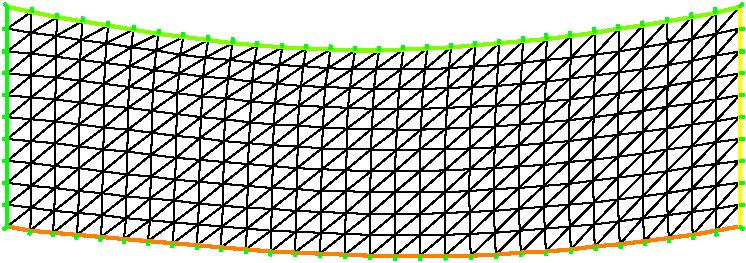
\includegraphics[width=16cm]{nl-elas}\end{center}
\caption{\label{fig nl-elas} The deformated domain}
\end{figure}



\end{document}